\documentclass[aspectratio=169]{beamer}
\newcommand{\sourcepath}[1]{../#1}
%\newcommand{\stylepath}[1]{../beamer/#1}


\usepackage{\sourcepath{beamer/beamerthemeLCS27}}
%\usepackage{indentfirst}

\background{../fig/BeihangPicture.jpg}
\schoollogo{../fig/BeihangLogo.jpg}
%\lablogo{../fig/CentraleSupelecRVB.jpg}


\author[]{罗宸晟}
\title{标题}
\institute{北京航空航天大学中法工程师学院/国际通用工程师学院 \\ 数理实验室-复杂系统实验室}
\date{\today}

\usepackage{lipsum} % for dummy text
\usepackage{zhlipsum} 

\begin{document}

\maketitle
\begin{frame}{目录}
\tableofcontents
\end{frame}
\section{章节一}
\begin{frame}[allowframebreaks]{标题一}{简述}
\zhlipsum[10]
\end{frame}

\section{章节二}
\begin{frame}[allowframebreaks]{标题二}{简述}
\zhlipsum[11]
\end{frame}
\begin{frame}[allowframebreaks]{标题三}{简述}
\zhlipsum[12]
\end{frame}

\section{章节三}

\begin{frame}[allowframebreaks]{标题四}{具体内容}
\zhlipsum[1]
\begin{figure}
    \centering
    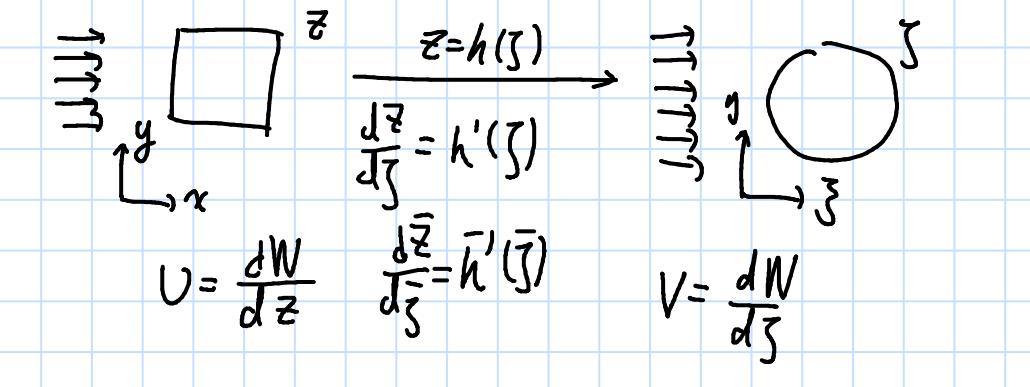
\includegraphics[width=0.5\textwidth]{../picture/1.jpg}
\end{figure}

\zhlipsum[2]
\begin{itemize}
    \item \zhlipsum[3]
    \item \zhlipsum[4]
    \item \zhlipsum[5]
\end{itemize}
\zhlipsum[6]
\end{frame}
\end{document}
